\documentclass{article}

\usepackage[parfill]{parskip}
\usepackage{
  geometry,
  float,
  listings,
  xcolor,
  amssymb,
  fontspec,
  graphicx,
  hyperref,
}

\graphicspath{ {../imgs/} }

% To keep figures, listings, and tables rendered where they're put
% *** BEGIN ***
\let\origfigure\figure
\let\endorigfigure\endfigure
\renewenvironment{figure}[1][2] {
    \expandafter\origfigure\expandafter[H]
} {
    \endorigfigure
}

\AtBeginDocument{\floatplacement{codelisting}{H}}
\AtBeginDocument{\floatplacement{table}{H}}
% *** END ***

\geometry{
  top = 20mm,
  bottom = 20mm,
  left = 25mm,
  right = 25mm,
  paper = a4paper,
}

\setmainfont{Times New Roman}
\setmonofont{JetBrainsMono Nerd Font Mono}

\definecolor{codegreen}{rgb}{0,0.6,0}
\definecolor{codegray}{rgb}{0.5,0.5,0.5}
\definecolor{codepurple}{rgb}{0.58,0,0.82}
\definecolor{backcolour}{rgb}{0.95,0.95,0.92}

\lstset{% https://en.wikibooks.org/wiki/LaTeX/Source_Code_Listings
  basicstyle = \footnotesize\ttfamily,
  breakatwhitespace = true,
  breaklines = true,
  frame = single,
  firstnumber = 1,
  keepspaces = true,
  numbers = left,
  tabsize = 4,
  backgroundcolor=\color{backcolour},
  commentstyle=\color{codegray},
  keywordstyle=\color{orange},
  numberstyle=\tiny\color{codegray},
  stringstyle=\color{codegreen},
  basicstyle=\ttfamily\footnotesize,
}

% https://github.com/gilangardya/if2211-cryptarithmetic-solver/blob/master/doc/LaporanTucil1.pdf

\begin{document}
\begin{titlepage}
  \centering
  \vspace*{\stretch{2}}
  \Large Laporan Tugas Kecil II

  \large Implementasi \textit{Topological Sort} dengan Menggunakan Pendekatan \textit{Decrease and Conquer}

  \normalsize

  \vspace{\stretch{1}}

  
\includegraphics[scale=0.2]{logo-itb.png}

  \vspace{\stretch{1}}
  \begin{tabular}{lll}
    Nama  &: & Josep Marcello \\
    NIM &: & 13519164 \\
    Kelas &: & K-03 \\
    Dosen &: & Prof.\ Dwi Hendratmo Widyantoro \\
    Bahasa &: & Java \\
  \end{tabular}

  \vspace{\stretch{2}}
  \large
  PROGRAM STUDI TEKNIK INFORMATIKA

  SEKOLAH TEKNIK ELEKTRO DAN INFORMATIKA

  INSTITUT TEKNOLOGI BANDUNG

  BANDUNG

  2021

  \vspace{\stretch{2}}
\end{titlepage}

\section{Algoritma \textit{Decrease and Conquer}}
Proses \textit{decrease and conquer} untuk topological sort dilakukan dengan
\textit{decrease by variable size}. Langkah-langkah algoritma \textit{decrease
and conquer}-nya adalah sebagai berikut:
\begin{enumerate}
  \item Lakukan partisi pada graf, misal $G_1 = (V_1, E_1)$, dengan
    pertama-tama mencari sudut-sudut di graf yang memiliki derajat masuk 0 atau
    $d_{in}(V_i) =~0$.
  \item Partisikan $G_1$ menjadi sebuah senarai dan graf baru, misal graf $G_1'
    = (V_1', E_1')$.  Senarai berisi sudut dari graf yang memiliki derajat
    masuk 0, sedangkan graf baru berisi sudut-sudut pada graf awal dikurangi
    sudut yang memiliki derajat masuk 0.
  \item Lakukan kembali langkah-langkah sebelumnya untuk $G_1'$ sampai dengan
    $|V_1'| = 0$.
  \item Masukkan senarai-senarai dari langkah 1--3 ke sebuah senarai dari
    senarai dari simpul secara berurutan dari iterasi pertama.
  \item Senarai baru adalah hasil \textit{topological sort} yang sudah
    diurutkan.
\end{enumerate}

\section{\textit{Source Code} Program}
\begin{lstlisting}[caption = App.java, language = java]
package Uranaishi;

import Uranaishi.lib.*;
import java.io.FileNotFoundException;
import java.io.IOException;
import java.util.ArrayList;
import java.util.Scanner;

/**
 * Berkas java utama untuk aplikasi Uranishi
 * @author Josep Marcello
 * 25 Februari 2021
 */
public class App {
    private static void printResult(ArrayList<ArrayList<Node>> nodes) {
        int i = 1;
        for (ArrayList<Node> vertList : nodes) {
            System.out.print("Semester " + i + ": ");
            int j = 0;
            for (Node node : vertList) {
                if (j != vertList.size()-1) {
                    System.out.print(node.getInfo() + ", ");
                } else {
                    System.out.print(node.getInfo());
                }
                ++j;
            }
            System.out.println();
            ++i;
        }
    }
    public static void main(String[] args) throws IOException, FileNotFoundException {
        //System.out.println("current working directory: " + System.getProperty("user.dir"));
        Scanner scan = new Scanner(System.in);
        Parser fp = null;
        Graph g1 = new Graph();

        // buat ngebaca argument dari user
        if (args.length != 0) {
            for (int i = 0; i < args.length; ++i) {
                if (args[i].equals("-f") || args[i].equals("--file")) {
                    fp = new Parser(args[++i]);
                } else if (args[i].equals("--help") || args[i].equals("-h")) {
                    System.out.println("uranaishi [nama jar] [--file|-f file-name] [--help|-h]");
                    System.out.println("\t-f\t--file\tArgumen ini diikuti path ke file yang berisi data graf.");
                    System.out.println("\t-h\t--help\tMenuliskan bantuan ini.");
                    System.exit(0);
                }
            }
        }

        // Ngebaca file kalo belom dibaca dari argumen
        if (fp == null) {
            System.out.print("Tuliskan path ke file yang berisi data graf: ");
            String input = scan.nextLine();
            fp = new Parser(input);
        }

        fp.openFile();
        g1 = fp.parse();
        scan.close();
        fp.close();

        System.out.println("Graf masukan:\n");
        g1.print();

        System.out.println("\n----------------------------\n");
        System.out.println("Hasil topological sort:\n");

        long start = System.nanoTime();
        ArrayList<ArrayList<Node>> nodes = g1.topoSort(0);
        long elapsedTime = System.nanoTime() - start;
        printResult(nodes);
        System.out.println("\nWaktu untuk memproses graf: " + elapsedTime + " nanodetik.");
        g1.print();
    }
}
\end{lstlisting}
\begin{lstlisting}[caption = lib/Node.java, language = java]
package Uranaishi.lib;

/**
 * Kelas yang merepresentasikan node (sudut) pada graf
 * @author Josep Marcello
 * 25 Februari 2021
 */
public class Node {
    // *** attribute ***
    private String info;

    // *** Getters and setters ***
    /**
     * Getter info attribute
     * @return info (nama) node
     */
    public String getInfo() {
        return this.info;
    }

    // *** Methods **
    /**
     * Konstruktor untuk class Node
     * @param info isi (nama) node
     */
    public Node(String info) {
        this.info = info;
    }

    /**
     * Fungsi untuk membandingkan node "this" dengan node lain
     * @param n2 node lain yang ingin dibandingkan dengan node "this"
     * @return true jika kedua node sama, false jika tidak
     */
    @Override
    public boolean equals(Object o) {
        if (o == null) {
            return false;
        }
        if (o.getClass() != this.getClass()) {
            return false;
        }

        Node n2 = (Node) o;
        return info.equals(n2.info);
    }

    /**
     * Fungsi untuk meng-override fungsi hashcode sehingga Node dapat digunakan
     * untuk key pada collection Map
     */
    @Override
    public int hashCode() {
        return this.info.hashCode();
    }
}
\end{lstlisting}
\begin{lstlisting}[caption = lib/Graph.java, language = java]
package Uranaishi.lib;

import java.util.HashMap;
import java.util.Iterator;
import java.util.ArrayList;

/**
 * Class yang merepresentasikan DAG yg memanfaatkan adjacency list
 * ({@link ArrayList}), {@link HashMap}, dan {@link Node}
 * @author Josep Marcelo
 * 25 Februari 2021
 */
public class Graph {
    // *** attribute ***
    /// adjacency list untuk graf
    private HashMap<Node, ArrayList<Node>> inEdges;

    // *** Getters and setters ***

    // *** Methods **
    /**
     * Konstruktor graf kosong
     */
    public Graph() {
        inEdges = new HashMap<>();
    }

    /**
     * Konstruktor graf berisi
     * Graf yang dibentuk adalah DAG dengan sisi e dan sudut v
     * @param v sisi-sisi pada DAG
     * @param e informasi sudut pada DAG [src vertex, dest vertex], pasti
     * berukuran [n][2], n sebuah integer
     */
    public Graph(Node[] v, Node[][] e) {
        inEdges =  new HashMap<>();
        for (Node[] adjNodes : e) {
            // add edge otomatis nambahin vertex kalo vertex-nya belom ada
            addEdge(adjNodes[0], adjNodes[1]);
        }
    }

    /**
     ` Fungsi untuk menambahkan sebuah sisi berarah antara 2 sudut. Jika sudut
     * asal dan sudut tujuan sama, maka tidak akan dilakukan apa-apa. Selain
     * itu, jika sudut asal tidak ada di graf, maka akan ditambahkan secara
     * otomatis ke graf
     * @param src sudut asal
     * @param dest sudut tujuan
     */
    public void addEdge(Node src, Node dest) {
        if (src != dest) {
            ArrayList<Node> adjList = inEdges.get(src);
            if (adjList == null) {
                adjList = new ArrayList<Node>();
                inEdges.put(src, adjList);
            }

            adjList.add(dest);
        }
    }

    /**
     * Fungsi untuk menambahkan sebuah sudut tanpa sisi ke graf. Jika sudut
     * sudah ada, tidak akan dilakukan apa-apa
     * @param n1 sudut yang akan ditambahkan ke graf
     */
    public void addVertex(Node n1) {
        if (!inEdges.containsKey(n1)) {
            inEdges.put(n1, new ArrayList<Node>());
        }
    }

    /**
     * Fungsi untuk menuliskan isi DAG (ditunjukkan sebagai adjacency list)
     */
    public void print() {
        for (Node vert: inEdges.keySet()) {
            ArrayList<Node> adjcentVertexes = inEdges.get(vert);
            int adjacentVertexCount = adjcentVertexes.size();

            // tulis vertex
            if (adjacentVertexCount != 0) {
                System.out.print(vert.getInfo() + "<-");
            } else {
                System.out.print(vert.getInfo());
            }

            // tulis sudut-sudut yang bertetanggaan dengan vertex
            int i = 0;
            for (Node adjacentVertex : adjcentVertexes) {
                if (i++ != adjacentVertexCount-1) {
                    System.out.print(adjacentVertex.getInfo() + "<-");
                } else {
                    System.out.print(adjacentVertex.getInfo());
                }
            }
            System.out.println();
        }
    }

    /**
     * Fungsi untuk menghapus sebuah vertex dari graf
     * @param n vertex yang ingin dihapus
     */
    private void removeVertex(Node n) {
        // iterasi key-nya
        Iterator<Node> itV = inEdges.keySet().iterator();
        while (itV.hasNext()) {
            Node vert = itV.next();
            ArrayList<Node> adjVerts = inEdges.get(vert);

            // kalau key-nya adalah elemen yang mau di-remove, remove vertex
            if (vert.equals(n)) {
                itV.remove();
            }

            // iterasi adjacency list setiap sudut
            Iterator<Node> itN = adjVerts.iterator();
            while(itN.hasNext()) {
                Node adjVert = itN.next();
                if (adjVert.equals(n)) {
                    // hapus kalo ada vertex n di dalem adjacency list
                    itN.remove();
                }
            }
        }
    }

    /**
     * Fungsi untuk mengurutkan graf dengan topological sort. PERHATIAN: fungsi
     * ini akan menghapus isi graf.
     * @return Urutan vertexes berdasarkan requirements yang sudah
     * dipisah-pisah
     */
    public ArrayList<ArrayList<Node>> topoSort(int iteration) {
        if (inEdges.isEmpty() || iteration == 10) {
            return new ArrayList<ArrayList<Node>>();
        }

        ArrayList<Node> takenNow = new ArrayList<>();
        ArrayList<ArrayList<Node>> ret = new ArrayList<>();

        // iterasiin vertices-nya
        for (Node vert: inEdges.keySet()) {
            ArrayList<Node> adjVert = inEdges.get(vert);

            // kalo ga ada adjacent vertex, tambahin vertex tadi ke list
            if (adjVert.isEmpty()) {
                takenNow.add(vert);
            }
        }

        // hapus vertex yang sudah "diambil"
        // bagian decrease
        for (Node vert : takenNow) {
            removeVertex(vert);
        }

        ret.add(takenNow);
        // ulangi toposort
        // bagian conquer
        ret.addAll(topoSort(++iteration));

        return ret;
    }
}
\end{lstlisting}
\begin{lstlisting}[caption = lib/Parser.java, language = java]
package Uranaishi.lib;

import java.io.BufferedReader;
import java.io.FileNotFoundException;
import java.io.FileReader;
import java.io.IOException;

/**
 * Class yang digunakan untuk parsing file yang mengandung data {@link Graph}
 * menjadi {@link Graph} sungguhan
 * @author Josep Marcello
 * 25 Februari 2021
 */
public class Parser {
    // *** attribute ***
    String pathToFile;
    FileReader fileReader;
    BufferedReader bufRead;

    // *** Methods ***
    /**
     * Konstruktor parser
     * @param path path ke file yang ingin di parse
     */
    public Parser(String path) {
        pathToFile = path;
    }

    /**
     * Fungsi untuk menge-parse 1 baris dari file menjadi {@link Node} untuk
     * {@link Graph}
     * @param line baris yang ingin di-parse menjadi {@link Node}
     * @return array of array of {@link Node} yang mengandung sudut "utama" di
     * indeks 0 dan sudut yang bertetanggaan di indeks 1. Ukurannya adalah
     * [2][n], n = 1 jika indeks 0, n = bilangan bulat jika indeks 1
     */
    private Node[][] parseLine(String line) {
        Node vertex;

        // Pisahin pada ", "
        String[] vertexesStrings = line.split(", ");

        // ngehapus titik dari vertex kalo ada
        String[] tmp = vertexesStrings[0].split("\\.");
        if (tmp.length == 1) {
            vertex = new Node(tmp[0]);
        } else {
           vertex = new Node(vertexesStrings[0]);
        }

        // ngehapus titik dari adjacent vertex terakhir
        int i = 1;
        int len = vertexesStrings.length;
        Node[] adjVert = new Node[vertexesStrings.length-1];
        for (; i < len; ++i) {
            // ngehapus titik dari adjacent vertex terakhir
            String[] vs = vertexesStrings[i].split("\\.");
            if (vs.length != 0) {
                adjVert[i-1] = new Node(vs[0]);
            } else {
                adjVert[i-1] = new Node(vertexesStrings[i]);
            }
        }

        Node[][] ret = { {vertex}, adjVert };

        return ret;
    }

    /**
     * Fungsi untuk membuka file dan memasukkanya ke {@link BufferedReader}
     * @throws FileNotFoundException {@link FileNotFoundException}
     * @throws IOException {@link IOException}
     */
    public void openFile() throws FileNotFoundException, IOException {
        fileReader = new FileReader(pathToFile);
        bufRead = new BufferedReader(fileReader);
    }

    /**
     * Fungsi untuk parsing file menjadi {@link Graph}
     * @return {@link Graph} dari hasil bacaan file
     * @throws IOException {@link IOException}
     */
    public Graph parse() throws IOException {
        Graph ret = new Graph();

        String line = bufRead.readLine();
        while (line != null) {
            if (line.length() != 0) {
                Node[][] lineParsed = parseLine(line);
                Node vertex = lineParsed[0][0];
                Node[] adjVert = lineParsed[1];

                ret.addVertex(vertex);
                for (Node adj : adjVert) {
                    ret.addEdge(vertex, adj);
                }
            }
            line = bufRead.readLine();
        }

        return ret;
    }

    /**
     * Fungsi untuk menutup {@link BufferedReader} dan {@link FileReader} pada
     * Parser
     * @throws IOException {@link IOException}
     */
    public void close() throws IOException {
        bufRead.close();
        fileReader.close();
    }
}
\end{lstlisting}

\section{Hasil Pengujian}
\subsection{Pengujian Pertama}
%\begin{lstlisting}[caption = \textit{input}]
%C1, C3.
%C2, C1, C4.
%C3.
%C4, C1, C3.
%C5, C2, C4.
%\end{lstlisting}
\begin{figure}
  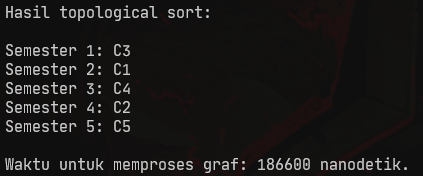
\includegraphics[scale=0.8]{1.png}
  \caption{\textit{input}}
\end{figure}
\begin{lstlisting}[caption = \textit{output}]
Hasil topological sort:

Semester 1: C3
Semester 2: C1
Semester 3: C4
Semester 4: C2
Semester 5: C5

Waktu untuk memproses graf: 115700 nanodetik.
\end{lstlisting}
\subsection{Pengujian Kedua}
\begin{lstlisting}[caption = \textit{input}]
Kriptografi, Matdis.
Kalkulus.
TBFO, Matdis.
Fisika.
Stima, Matdis, Kalkulus.
Matdis, Kalkulus.
\end{lstlisting}
%\begin{lstlisting}[caption = \textit{output}]
%Hasil topological sort:

%Semester 1: Fisika, Kalkulus
%Semester 2: Matdis
%Semester 3: TBFO, Stima, Kriptografi

%Waktu untuk memproses graf: 113800 nanodetik.
%\end{lstlisting}
\begin{figure}
  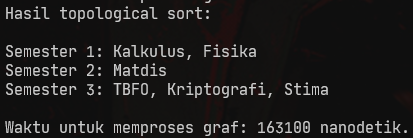
\includegraphics[scale=0.8]{2.png}
  \caption{\textit{input}}
\end{figure}
\subsection{Pengujian Ketiga}
\begin{lstlisting}[caption = \textit{input}]
MA1201, MA1101.
FI1201, FI1101.
IF1210, KU1102.
KU1202, KU1102.
KI1002, KU1011.
EL1200, FI1101.
KU1102.
MA1101.
FI1101.
KU1011.
\end{lstlisting}
%\begin{lstlisting}[caption = \textit{output}]
%Hasil topological sort:

%Semester 1: KU1102, KU1011, MA1101, FI1101
%Semester 2: IF1210, KI1002, EL1200, MA1201, KU1202, FI1201

%Waktu untuk memproses graf: 178000 nanodetik.
%\end{lstlisting}
\begin{figure}
  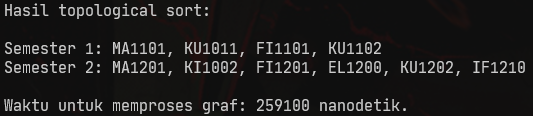
\includegraphics[scale=0.8]{3.png}
  \caption{\textit{input}}
\end{figure}
\subsection{Pengujian Keempat}
\begin{lstlisting}[caption = \textit{input}]
MA1101.
FI1101.
KU1001.
KU1102.
KU1011.
KU1024.
MA1201, MA1101.
FI1201, FI1101.
IF1210.
KU1202.
EL1200, MA1101.
IF2121.
IF2110.
IF2120.
IF2124.
IF2123, MA1101.
IF2130.
IF2210, IF2110.
IF2211.
IF2220, MA1101, MA1201, IF2120.
IF2230.
IF2240.
IF2250.
IF3170, IF2121, IF2124, IF2220, IF2211.
IF3110, IF2210, IF2110.
IF3130, IF2230.
IF3141, IF2240, IF2250.
IF3150, IF2250.
IF3140.
IF3151, IF2250.
IF3210, IF2130, IF2110.
IF3270, IF3170, IF2110.
IF3230, IF3130.
IF3250, IF3150, IF2250.
IF3260, IF2130, IF2110, IF2123.
IF3280.
IF4090, IF3280.
IF4091.
KU2071.
IF4092, IF4091.
KU206X.
AS2005.
\end{lstlisting}
%\begin{lstlisting}[caption = \textit{output}]
%Hasil topological sort:

%Semester 1: IF3280, IF2121, KU1001, KU1024, AS2005, IF4091, MA1101, KU2071, KU1102, IF2250, IF1210, IF2240, KU206X, IF3140, KU1011, KU1202, IF2120, IF2230, IF2110, IF2130, IF2124, FI1101, IF2211
%Semester 2: MA1201, IF2210, IF4090, FI1201, IF3150, IF4092, IF3210, IF3130, IF2123, IF3141, IF3151, EL1200
%Semester 3: IF2220, IF3230, IF3250, IF3260, IF3110
%Semester 4: IF3170
%Semester 5: IF3270

%Waktu untuk memproses graf: 1129700 nanodetik.
%\end{lstlisting}
\begin{figure}
  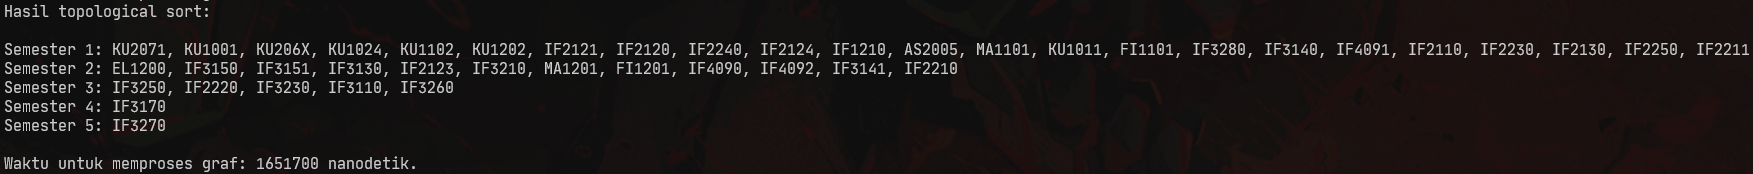
\includegraphics[scale=0.25]{4.png}
  \caption{\textit{input}}
\end{figure}
\subsection{Pengujian Kelima}
\begin{lstlisting}[caption = \textit{input}]
Flask, Python, Pip.
Pip, Python.
Python, C.
C.
\end{lstlisting}
%\begin{lstlisting}[caption = \textit{output}]
%Hasil topological sort:

%Semester 1: C
%Semester 2: Python
%Semester 3: Pip
%Semester 4: Flask

%Waktu untuk memproses graf: 101700 nanodetik.
%\end{lstlisting}
\begin{figure}
  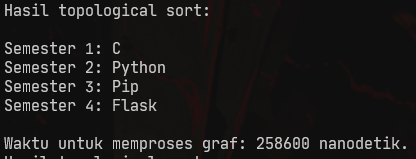
\includegraphics[scale=0.7]{5.png}
  \caption{\textit{input}}
\end{figure}
\subsection{Pengujian Keenam}
\begin{lstlisting}[caption = \textit{input}]
MA1101.
FI1101.
KU1001.
KU1102.
KU1011.
KU1024.

MA1201, MA1101.
FI1201, FI1101.
IF1210, KU1102.
KU1202, KU1102.
KI1002, KU1011.
EL1200, FI1101.

IF2121, IF1210, MA1101, MA1201.
IF2110, KU1102, IF1210.
IF2120, MA1201, MA1101.
IF2124, EL1200.
IF2123, MA1201.
IF2130, KU1202.

IF2210, IF2110.
IF2211, IF2110.
IF2220, MA1101, MA1201, IF2120.
IF2230, IF2130.
IF2240, IF2121, IF2120.
IF2250, KU1202, IF2110.

IF3170, IF2121, IF2124, IF2220, IF2211.
IF3110, IF2210, IF2110.
IF3130, IF2230.
IF3141, IF2240, IF2250.
IF3150, IF2250.
IF3140, IF2240.
IF3151, IF2250.

IF3210, IF2110, IF2130, IF3110.
IF3270, IF2210, IF3170.
IF3230, IF3130.
IF3250, IF2250, IF3150.
IF3260, IF2123, IF2110, IF2130, IF3151.
IF3280, IF3151, IF3150.

IF4090, IF3280.
IF4091, IF3280.

IF4092, IF4091.
\end{lstlisting}
%\begin{lstlisting}[caption = \textit{output}]
%Hasil topological sort:

%Semester 1: KU1001, KU1024, MA1101, KU1102, KU1011, FI1101
%Semester 2: EL1200, MA1201, IF1210, KU1202, FI1201, KI1002
%Semester 3: IF2130, IF2110, IF2124, IF2121, IF2123, IF2120
%Semester 4: IF2211, IF2240, IF2230, IF2220, IF2250, IF2210
%Semester 5: IF3150, IF3141, IF3151, IF3110, IF3130, IF3140, IF3170
%Semester 6: IF3260, IF3270, IF3210, IF3230, IF3280, IF3250
%Semester 7: IF4090, IF4091
%Semester 8: IF4092

%Waktu untuk memproses graf: 1668500 nanodetik.
%\end{lstlisting}
\begin{figure}
  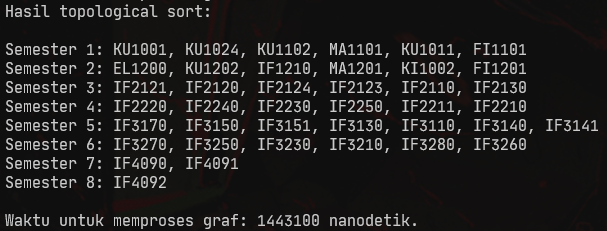
\includegraphics[scale=0.7]{6.png}
  \caption{\textit{input}}
\end{figure}
\subsection{Pengujian Ketujuh}
\begin{lstlisting}[caption = \textit{input}]
A.
full.
commitments.
what.
i'm.
thinking.
of.
You, full.
wouldn't, what.
get, A.
this, thinking.
from, what.
any, thinking.
other, of.
guy, A.
I, wouldn't.
just, thinking, this.
wanna, A, full, guy.
tell, You.
you, wouldn't, get.
how, wouldn't.
I'm, thinking, of, You.
feeling, You, wouldn't, commitments.
Gotta, get, this, feeling.
make, you, thinking.
u, wanna, tell, feeling.
understand, you.
Never, thinking, of, u.
gonna, make, u, understand.
give, u, feeling.
U, Gotta, understand.
up, of, u.
never, make, You, thinking, Never.
Gonna, make, u, understand, U, Never, give, up.
let, feeling, make, you, give, up.
yOu, wanna, tell, feeling, give, up.
down, Never, make.
\end{lstlisting}
%\begin{lstlisting}[caption = \textit{output}]
%Hasil topological sort:

%Semester 1: of, commitments, thinking, A, what, i'm, full
%Semester 2: from, wouldn't, get, You, other, any, guy, this
%Semester 3: you, feeling, wanna, I'm, how, I, just, tell
%Semester 4: u, understand, Gotta, make
%Semester 5: up, gonna, Never, U, give
%Semester 6: yOu, never, Gonna, down, let

%Waktu untuk memproses graf: 1146200 nanodetik.
%\end{lstlisting}
\begin{figure}
  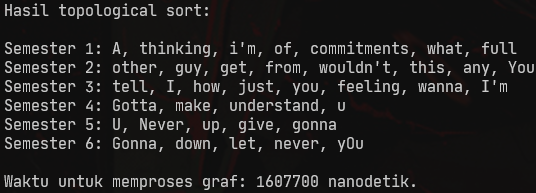
\includegraphics[scale=0.7]{7.png}
  \caption{\textit{input}}
\end{figure}
\subsection{Pengujian Kedelapan}
\begin{lstlisting}[caption = \textit{input}]
nodemon, chokidar, glob-parent, debug, ignore-by-default, minimatch, pstree, semver, supports-color, touch, undefsafe, update-notifier.
update-notifier, boxen, chalk, configstore, has-yarn, import-lazy, is-ci, is-installed-globally, is-npm, is-yarn-global, latest-version, pupa, semver-diff, xdg-basedir.
chokidar, anymatch, braces, fsevents, glob-parent, is-binary-path, is-glob, normalize-path, readdirp.
fsevents.
anymatch, normalize-path, picomatch.
normalize-path.
picomatch.
braces, fill-range.
fill-range, to-regex-range.
to-regex-range, is-number.
is-number.
glob-parent, is-glob.
is-glob, is-extglob.
is-extglob
is-binary-path, binary-extensions.
binary-extensions.
readdirp, picomatch.
debug, ms.
ms.
minimatch, brace-expansion.
brace-expansion, balanced-match, concat-map.
balanced-match.
concat-map.
ignore-by-default.
pstree.
semver.
supports-color, has-flag.
has-flag.
touch, nopt.
nopt, abbrev.
abbrev.
undefsafe, debug.
boxen, ansi-align, camelcase, chalk, cli-boxes, string-width, term-size, type-fest, widest-line.
camelcase.
ansi-align, string-width.
string-width, emoji-regex, is-fullwidth-code-point, strip-ansi.
emoji-regex.
is-fullwidth-code-point.
strip-ansi, ansi-regex.
ansi-regex.
chalk, ansi-styles, supports-color.
ansi-styles, @types/color-name, color-convert.
@types/color-name.
color-convert, color-name.
color-name.
has-flag.
cli-boxes.
term-size.
type-fest.
widest-line, string-width.
configstore, dot-prop, graceful-fs, make-dir, unique-string, write-file-atomic, xdg-basedir.
dot-prop, is-obj.
is-obj.
graceful-fs.
make-dir, semver.
unique-string, crypto-random-string.
crypto-random-string.
write-file-atomic, imurmurhash, is-typedarray, signal-exit, typedarray-to-buffer.
imurmurhash.
is-typedarray.
signal-exit.
typedarray-to-buffer, is-typedarray.
xdg-basedir.
has-yarn.
import-lazy.
is-ci, ci-info.
ci-info.
is-installed-globally, global-dirs, is-path-inside.
global-dirs, ini.
ini.
is-path-inside.
is-npm.
is-yarn-global.
pupa, escape-goat.
escape-goat.
semver-diff, semver.
latest-version, package-json.
package-json, got, registry-auth-token, registry-url, semver.
registry-url, rc.
rc, deep-extend, ini, minimist, strip-json-comments.
deep-extend.
minimist.
strip-json-comments.
registry-auth-token, rc.
got, @sindresorhus/is, @szmarczak/http-timer, cacheable-request, decompress-response, duplexer3, get-stream, lowercase-keys, mimic-response, p-cancelable, to-readable-stream.
@sindresorhus/is.
duplexer3.
lowercase-keys.
mimic-response.
p-cancelable.
to-readable-stream.
url-parse-lax, prepend-http.
prepend-http.
get-stream, pump.
pump, end-of-stream, once.
end-of-stream, once.
once, wrappy.
wrappy.
decompress-response, mimic-response.
cacheable-request, clone-response, get-stream, http-cache-semantics, keyv, lowercase-keys, normalize-url, responselike.
responselike, lowercase-keys.
normalize-url.
keyv, json-buffer.
json-buffer.
http-cache-semantics.
get-stream, pump.
clone-response, mimic-response.
mimic-response.
@szmarczak/http-timer, defer-to-connect.
defer-to-connect.
\end{lstlisting}
%\begin{lstlisting}[caption = \textit{output}]
%Hasil topological sort:

%Semester 1: xdg-basedir, camelcase, term-size, emoji-regex, to-readable-stream, abbrev, escape-goat, minimist, p-cancelable, binary-extensions, ignore-by-default, strip-json-comments, ci-info, has-flag, is-fullwidth-code-point, defer-to-connect, fsevents, concat-map, color-name, balanced-match, graceful-fs, is-extglob, prepend-http, json-buffer, type-fest, is-typedarray, is-yarn-global, http-cache-semantics, lowercase-keys, wrappy, is-number, @sindresorhus/is, picomatch, signal-exit, mimic-response, is-path-inside, is-obj, ansi-regex, @types/color-name, semver, cli-boxes, normalize-url, imurmurhash, pstree, ms, is-npm, normalize-path, crypto-random-string, ini, duplexer3, has-flag, import-lazy, deep-extend, mimic-response, has-yarn
%Semester 2: semver-diff, to-regex-range, unique-string, dot-prop, supports-color, url-parse-lax, decompress-response, clone-response, rc, readdirp, color-convert, typedarray-to-buffer, keyv, debug, global-dirs, once, is-glob, @szmarczak/http-timer, strip-ansi, responselike, anymatch, brace-expansion, pupa, is-ci, make-dir, is-binary-path, nopt
%Semester 3: ansi-styles, registry-auth-token, touch, fill-range, string-width, glob-parent, registry-url, is-installed-globally, minimatch, end-of-stream, undefsafe, write-file-atomic
%Semester 4: configstore, pump, widest-line, braces, chalk, ansi-align
%Semester 5: boxen, get-stream, get-stream, chokidar
%Semester 6: cacheable-request
%Semester 7: got
%Semester 8: package-json
%Semester 9: latest-version
%Semester 10: update-notifier
%Semester 11: nodemon

%Waktu untuk memproses graf: 3478700 nanodetik.
%\end{lstlisting}
\begin{figure}
  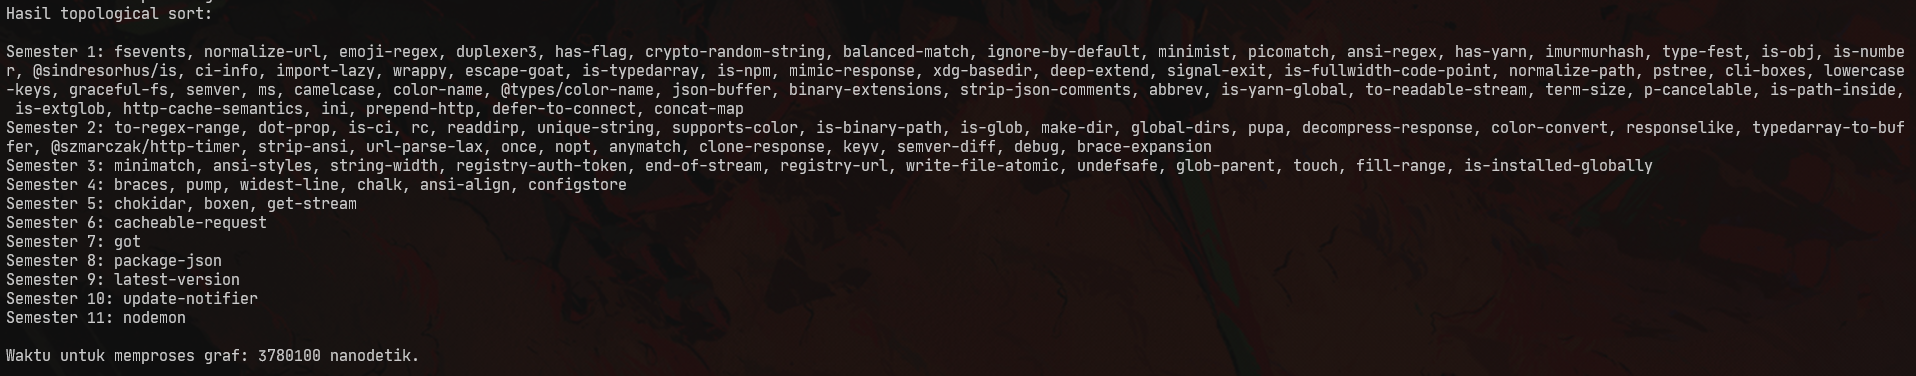
\includegraphics[scale=0.25]{8.png}
  \caption{\textit{input}}
\end{figure}

\subsection{Tabel Penilaian}
\begin{table}
  \begin{center}
    \begin{tabular}{|p{7cm} | l | l|}
      \hline
      Poin & Ya & Tidak \\
      \hline
      1. Program berhasil dikompilasi & \checkmark & \\
      \hline
      2. Program berhasil \textit{running} & \checkmark & \\
      \hline
      3. Program dapat menerima berkas input dan menuliskan output & \checkmark & \\
      \hline
      4. Luaran sudah benar untuk semua kasus input & \checkmark & \\
      \hline
    \end{tabular}
  \end{center}
\end{table}

\section*{\textit{Link} ke \textit{repository} Github}
\href{https://github.com/jspmarc/Tucil1_13519164}{\textit{Link} ke
\textit{repository}}: https://github.com/jspmarc/Uranaishi.

\end{document}
